\section{Performances :}
Tous les tests de performance présentés dans cette section ont été effectués sur un Nokia 3.1.
Voici un résumé de ses caractéristiques :
\begin{itemize} [label=\textbullet]
  \item \textbf{Version} : Android 9
  \item \textbf{Résolution}	: 1440 x 720 pixels
  \item \textbf{Cadence processeur} : 1.5 GHz
  \item \textbf{RAM} : 2 Go
\end{itemize}

\subsection{Temps d'exécution :}

Les temps d'exécution présentés ne tiennent pas compte du premier temps de chargement du script renderscript.
\\

Voici les temps d'exécution \textbf{sur 10 appels} de chaque effet pour une image de dimension \textbf{425x265px}.
\\

\begin{tabular}{||l||c|c||c|c||}
    \hline
    \hline
    \textbf{Effet} & \textbf{Temps d'exécution en ms} (min | max | moyenne | écart-type)\\
    \hline
    \hline
    Brightness & 12.0 | 46.0 | 16.9 | 9.73\\
    \hline
    Contrast & 16.0 | 28.0 | 20.5 | 3.80\\
    \hline
    Saturation & 13.0 | 23.0 | 15.2 | 2.929\\
    \hline
    Enhance & 22.0 | 32.0 | 26.4 | 3.00\\
    \hline
    To gray & 9.0 | 11.0 | 10.0 | 0.63\\
    \hline
    Invert & 8.0 | 10.0 | 8.4 | 0.66\\
    \hline
    Change hue & 11.0 | 18.0 | 13.4 | 1.90\\
    \hline
    Keep hue & 10.0 | 11.0 | 10.6 | 0.48\\
    \hline
    Gaussian blur 3x3 & 17.0 | 21.0 | 18.8 | 1.24\\
    \hline
    Gaussian blur 25x25 & 47.0 | 51.0 | 48.5 | 1.36\\
    \hline
    Mean blur 3x3 & 16.0 | 19.0 | 18.2 | 1.07\\
    \hline
    Mean blur 25x25 & 54.0 | 60.0 | 55.8 | 1.72\\
    \hline
    Sharpen 3x3 & 21.0 | 25.0 | 23.6 | 1.11\\
    \hline
    Sharpen 13x13 & 136.0 | 165.0 | 146.3 | 8.97\\
    \hline
    Sobel filter & 21.0 | 31.0 | 24.7 | 2.53\\
    \hline
    Prewitt filter & 24.0 | 27.0 | 25.3 | 1.09\\
    \hline
    Laplacian filter & 22.0 | 26.0 | 23.6 | 1.11\\
    \hline
    \hline
  \end{tabular}
\\
\newpage
Voici les temps d'exécution \textbf{sur 10 appels} de chaque effet pour une image de dimension \textbf{3400x2118px}.
\\

\begin{tabular}{||l||c|c||c|c||}
    \hline
    \hline
    \textbf{Effet} & \textbf{Temps d'exécution en ms} (min | max | moyenne | écart-type)\\
    \hline
    \hline
    Brightness & 105.0 | 311.0 | 145.8 | 56.95\\
    \hline
    Contrast & 163.0 | 202.0 | 176.9 | 12.73\\
    \hline
    Saturation & 209.0 | 236.0 | 221.4 | 8.34\\
    \hline
    Enhance & 256.0 | 268.0 | 261.3 | 3.74\\
    \hline
    To gray & 125.0 | 138.0 | 129.6 | 3.35\\
    \hline
    Invert & 84.0 | 105.0 | 94.7 | 8.69\\
    \hline
    Change hue & 218.0 | 319.0 | 231.7 | 29.48\\
    \hline
    Keep hue & 162.0 | 181.0 | 168.4 | 5.06\\
    \hline
    Gaussian blur 3x3 & 245.0 | 265.0 | 256.4 | 6.63\\
    \hline
    Gaussian blur 25x25 & 1453.0 | 1484.0 | 1462.2 | 9.08\\
    \hline
    Mean blur 3x3 & 245.0 | 652.0 | 358.5 | 146.25\\
    \hline
    Mean blur 25x25 & 1461.0 | 2447.0 | 1716.6 | 318.34\\
    \hline
    Sharpen 3x3 & 433.0 | 524.0 | 471.7 | 25.25\\
    \hline
    Sharpen 13x13 & 5112.0 | 8974.0 | 5679.2 | 1119.49\\
    \hline
    Sobel filter & 450.0 | 497.0 | 469.4 | 14.47\\
    \hline
    Prewitt filter & 452.0 | 490.0 | 472.5 | 10.39\\
    \hline
    Laplacian filter & 411.0 | 533.0 | 460.4 | 40.08\\
    \hline
    \hline
  \end{tabular}

\subsubsection*{Conclusion sur les temps d'exécution}

Mesurer les temps d'exécution nous a permis de nous rendre compte du gain de temps de la convolution séparable. Le flou gaussien (implémenté en séprable) 25x25 prend 1462.2 ms, tandis que le sharpen 13x13 (non séparable) prend 5679.2 ms.  

Sharpen 3x3, Sobel, Prewitt et Laplacian ont le même temps d'exécution car elles correspondent toutes à des convolutions classique avec un kernel 3x3.

De plus, on remarque que l'effet "Invert" est le plus rapide. Cela s'explique par le fait que c'est le seul effet qui manipule directement des entiers. Peut-être pourrions-nous appliquer cette méthode à d'autres effets tels que la convolution, afin d'optimiser les temps d'exécution.

\subsection{Mémoire :}

Voici l'utilisation de la mémoire vive du téléphone au cours de l'utilisation de l'application. On démarre le benchmarking à partir du chargement de l'image (après fistActivity), puis on applique tous les effets disponibles en annulant à chaque fois.
\subsubsection*{Image de 425x265px}
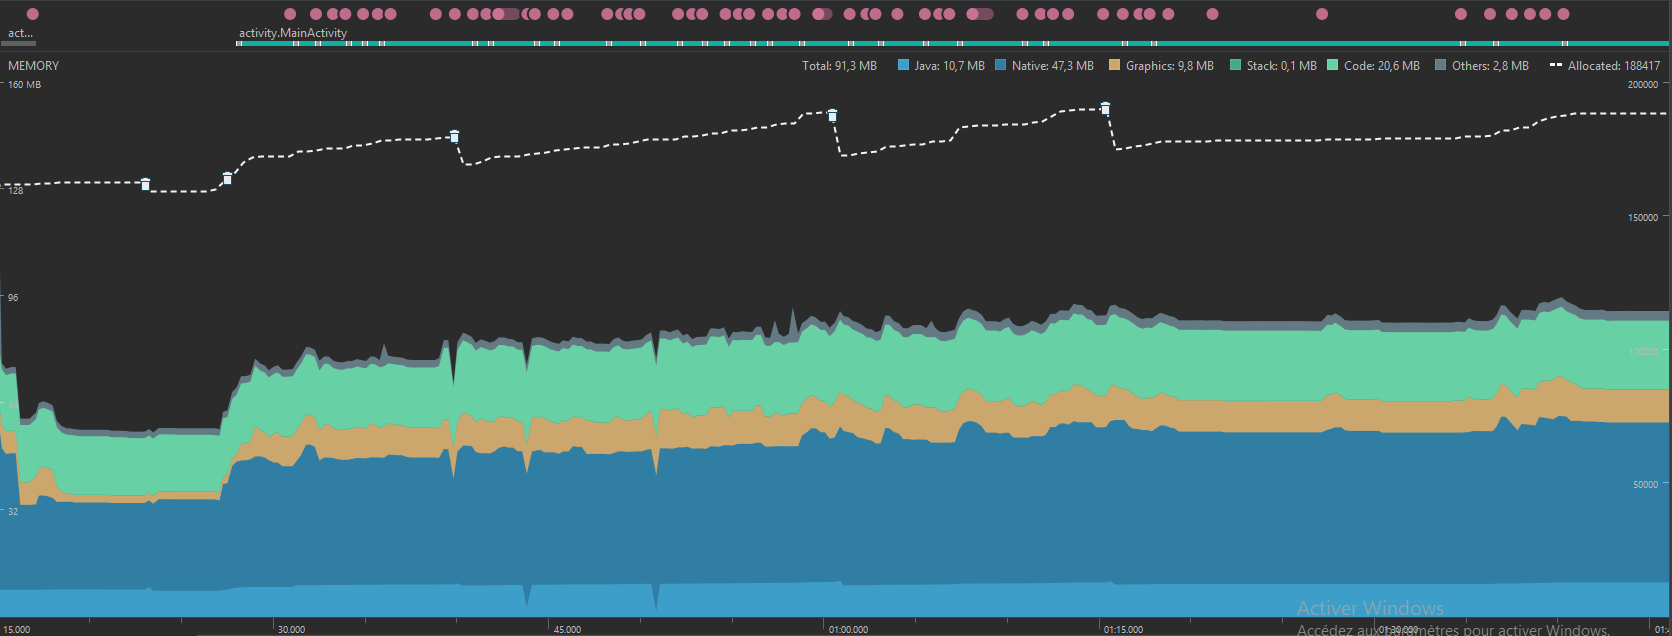
\includegraphics[width=1\textwidth]{report_src/memory/425x265.PNG}

\subsubsection*{Image de 3400x2118px}
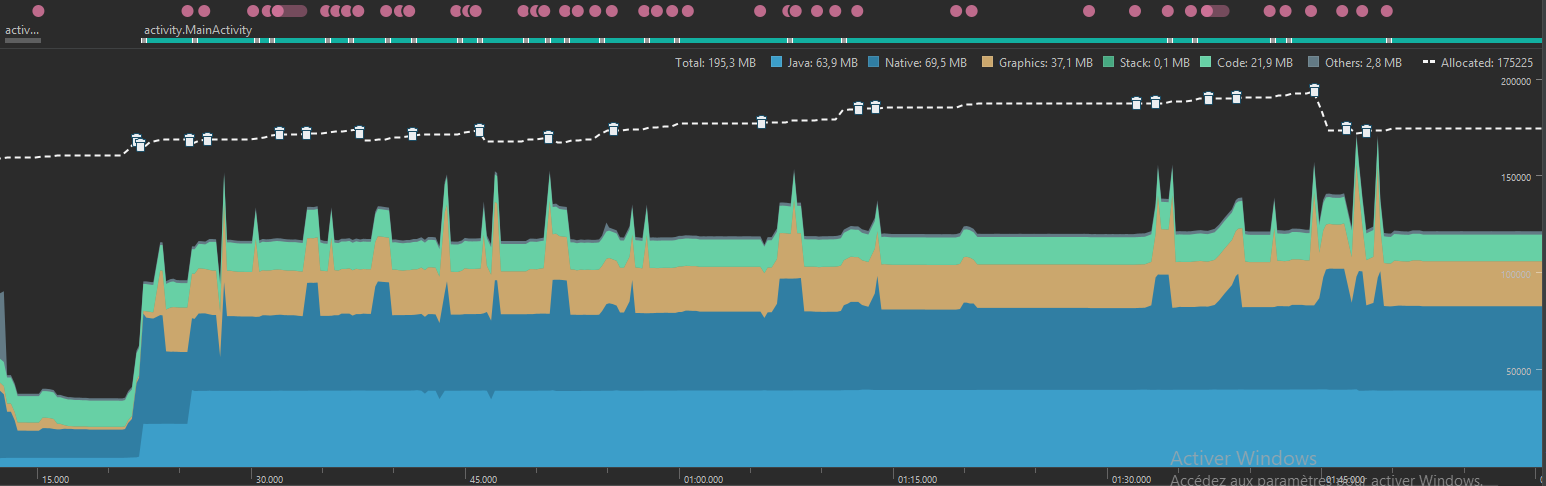
\includegraphics[width=1\textwidth]{report_src/memory/3400x2118.PNG}

\subsubsection*{Conclusion sur l'utilisation de la mémoire}
On observe que la mémoire est plutôt bien gérée et qu'elle reste constante tout au long de l'utilisation. De plus, le garbage collector vient régulièrement libérer la mémoire allouée.

En analysant le tas de l'application ("app heap" sur le profiler), on se rend compte que la sauvegarde de l'image (effectuée avec la méthode quicksave()) y occupe la plus grande place. La sauvegarde est stockée sous forme de tableau d'entiers, on peut donc difficilement le rendre moins lourd en mémoire. En revanche, la file d'effets (\textbf{\ref{file_effets}}) pourrait nous permettre d'annuler les modifications sans avoir à stocker une sauvegarde. En effet, si l'utilisateur a appliqué n effets et qu'il souhaite annuler la dernière modification, on peut ré-appliquer tous les effets jusqu'à n-1 sur l'image d'origine. Cependant, on perdrait évidemment en temps.

\newpage

\subsubsection*{Bug détecté}

Le profiling de la mémoire nous a permis de détecter un problème que l'on a résolu. En effet, on remarquait une augmentation constante de la mémoire lorsque l'on appliquait un flou :
\\

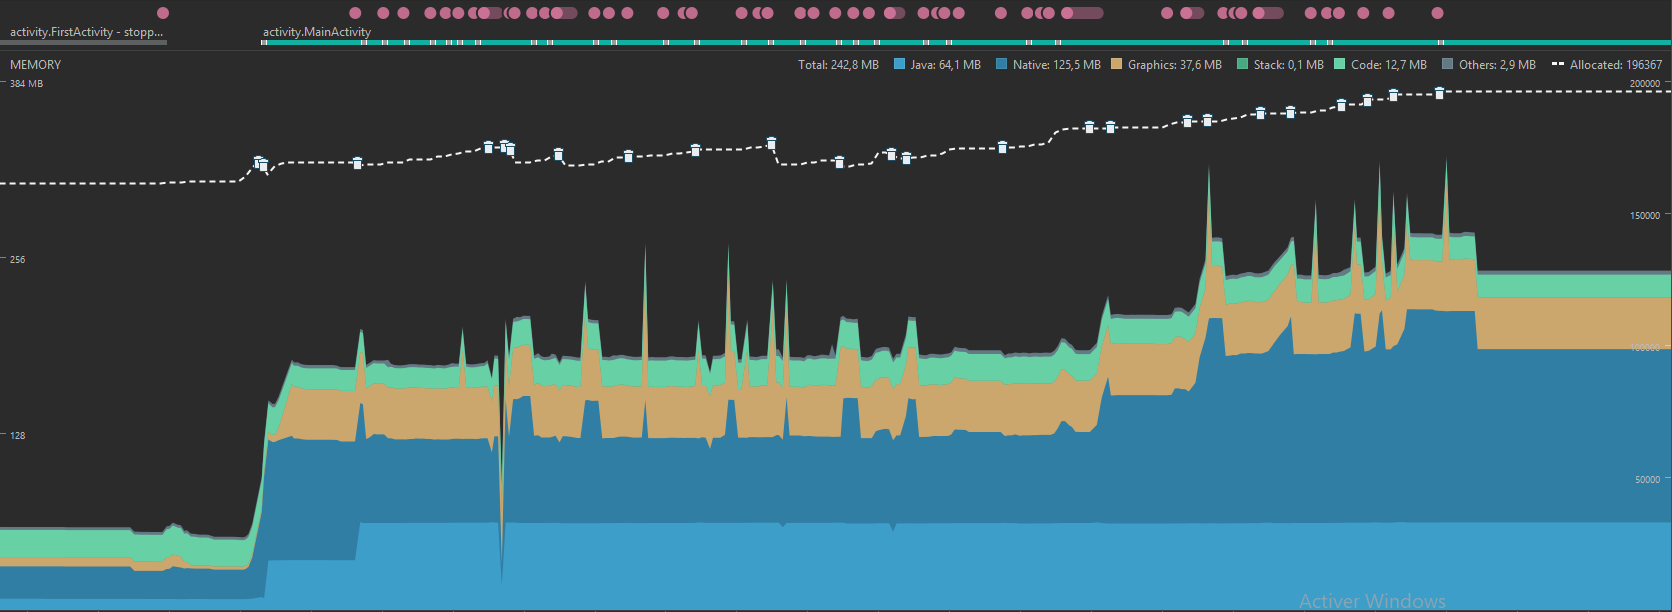
\includegraphics[width=1\textwidth]{report_src/memory/3400x2118_with_bug.PNG}
\\

C'était du à notre méthode convolve2dSeparable. La convolution séparée nécessite une allocation temporaire pour stocker le résultat de la première convolution (horizontale). 
Elle était créée puis libérée directement depuis notre script convolution.rs (méthode convolutionSeparable). Cependant, la libération ne fonctionnait apparemment pas, nous avons donc géré l'allocation de ce bitmap temporaire depuis java, ce qui a réglé le problème.
